\documentclass[11pt,a4paper]{article}

\usepackage[margin=1in]{geometry}
\usepackage{amsmath,amssymb}
\usepackage{booktabs,longtable,array,tabularx}
\usepackage{xltabular}
\usepackage{enumitem}
\usepackage{graphicx}
\usepackage{xcolor}
\usepackage{hyperref}
\usepackage{fancyhdr}
\usepackage[most]{tcolorbox}
\usepackage{tikz}
\usepackage{float}
\usetikzlibrary{arrows.meta,positioning,shapes.geometric,fit,calc}

\hypersetup{colorlinks=true,linkcolor=black,urlcolor=blue,citecolor=black}
\setlength{\parindent}{0pt}
\setlength{\parskip}{6pt}
\renewcommand{\arraystretch}{1.25}
\setlist{itemsep=2pt,topsep=3pt}

\pagestyle{fancy}
\fancyhf{}
\fancyfoot[C]{\hfill \thepage}
\renewcommand{\headrulewidth}{0pt}

\graphicspath{{../docs/figures/report/}{../docs/figures/}}

\newtcolorbox{keybox}[1]{colback=blue!4,colframe=blue!50!black,fonttitle=\bfseries,title=#1}
% Values that must be filled in after the final tag is created
\newcommand{\fillin}[1]{\textcolor{red}{[#1]}}

% Final tag; every evidence link below resolves to this revision
\newcommand{\finaltag}{cs5903-final-2026}
\newcommand{\repobase}{https://github.com/vhemanth06/AdaptEngine}
\newcommand{\repo}[1]{\href{\repobase/blob/\finaltag/#1}{\nolinkurl{#1}}}
\newcommand{\repodir}[1]{\href{\repobase/tree/\finaltag/#1}{\nolinkurl{#1}}}
\newcommand{\commit}[1]{\href{\repobase/commit/#1}{\texttt{#1}}}

\begin{document}

%-------------------------------------------------- Title page
\begin{titlepage}
\centering
\vspace*{1.5cm}
{\Large \textbf{IIT HYDERABAD}}\\[0.4cm]
{\large CS5903 -- Distributed AI Training}\\[1.5cm]
{\Huge \textbf{AdaptEngine}}\\[0.5cm]
{\Large Project 03: Adaptive Learning, Diagnostic Assessment and\\ Personalized Path-Planning Engine}\\[1.5cm]
{\LARGE \textbf{Final Project Report}}\\[1.5cm]
{\large Vuppula Hemanth Reddy\\[0.2cm]
AI23BTECH11033\\[0.2cm]
Group 15}\\[1.5cm]
{\large Repository: \url{https://github.com/vhemanth06/AdaptEngine}}\\[0.3cm]
{\large Final tag: \texttt{\finaltag} \quad Commit: \fillin{final commit SHA}}\\[0.3cm]
{\large Demo: local only, \texttt{make demo} $\rightarrow$ \url{http://127.0.0.1:8000}}
\vfill
{\small Report date: 15 November 2026. All learners in the evaluation are simulated.}
\end{titlepage}

%-------------------------------------------------- Executive summary
\section*{Executive Summary}
\addcontentsline{toc}{section}{Executive Summary}

\begin{keybox}{Summary}
\textbf{Problem.} Online courses give every learner the same lesson order. AdaptEngine instead finds out what a learner knows, plans what to study within a goal, a deadline and a daily budget of 5--30 minutes, adapts after every answer or disruption, and explains each decision.

\textbf{Delivered solution.} A deterministic Python engine (version 1.0.0): a reviewed prerequisite graph, a BKT mastery model, an adaptive goal-path diagnostic, a budgeted planner with an exact feasibility oracle, spaced review and remediation, replanning for four event types, and a decision trace for every planned activity. A FastAPI adapter and an 11-screen React web app sit on top. An optional agentic layer (bandit ranker, authoring aid, plan proposer, orchestrator) is off by default.

\textbf{What works today.} All 23 acceptance tests in the register have automated tests; 22 pass and the TC2.1 accuracy clause is not met. In the pre-registered product rerun, every adaptive arm had \textbf{0 prerequisite and 0 budget violations} over 462,600 simulated episodes. Replanning is essential (no-replan is $-0.411$ goal mastery in the headline cell).

\textbf{Overall state.} Complete prototype; evaluation is synthetic only. The shipped product configuration is safe but does \emph{not} beat a state-blind practice loop on goal mastery in most cells (15 better, 45 no difference, 148 worse of 208).
\end{keybox}

\tableofcontents
\newpage

%==================================================== 1
\section{Problem, Scope and Success Criteria}

\subsection{Users and problem statement}

The users are (i) a \textbf{learner} who has a goal concept, a deadline and a fixed number of free minutes each day, (ii) a \textbf{content author} who writes the curriculum, and (iii) an \textbf{evaluator or developer} who runs the engine through the CLI, the Python API or the simulator.

The problem is the one stated in the mid report. A fixed lesson order cannot suit both a beginner with 10 minutes a day and an experienced learner who wants a short refresher. The engine must:
\begin{itemize}
\item estimate the starting mastery of each concept from a short diagnostic, with uncertainty;
\item never break a prerequisite or the daily budget, and say clearly when a goal cannot fit;
\item share one budget between new lessons, remediation and spaced review;
\item replan after a missed day, a failed assessment, or a change of deadline or budget, without losing completed work;
\item explain every inclusion, omission and difficulty choice.
\end{itemize}

\subsection{Scope}

\begin{xltabular}{\textwidth}{
    @{}
    >{\raggedright\arraybackslash}p{0.48\textwidth}
    >{\raggedright\arraybackslash}X
    @{}
}
\caption{In and out of scope.}
\label{tab:scope}\\
\toprule
\textbf{In scope} & \textbf{Out of scope} \\
\midrule
\endfirsthead
\toprule
\textbf{In scope} & \textbf{Out of scope} \\
\midrule
\endhead
\bottomrule
\endfoot
Any subject that can be written as a prerequisite DAG with binary-graded exercises; demonstrated on small Python curricula (4 and 8 concepts) and synthetic 20- and 50-concept curricula. & A full learning platform, user accounts, real course authoring at scale. \\
Python API, CLI, local FastAPI adapter and React demo app. & Hosted deployment, authentication, multi-user data. \\
Simulated learners in six worlds (S0--S4, S4F) with pre-registered protocols. & Real learner data, classroom pilot, private learner records. \\
Optional agents behind flags, tested offline with stubs. & Live LLM evaluation (no model was connected for the evaluation). \\
\end{xltabular}

\subsection{Assumptions and constraints}

The prerequisite graph is an accurate DAG with hard edges. Activities have fixed, indivisible integer durations, and a missed day means zero minutes. Each exercise maps to exactly one concept, has a difficulty $d\in[0.05,0.95]$, and is graded strictly correct or wrong. The core must be deterministic: no wall clock, no global random state, and no network access. Every result must carry a code hash so it can be traced to the exact source.

\subsection{Approved milestones and done-when criteria}

The milestones M1--M8 and the 23 acceptance tests were frozen in Assignment~2 and in the mid report; they are unchanged. The project-specific workflow is \emph{done when} a learner session can go through \emph{load reviewed content $\rightarrow$ diagnose $\rightarrow$ plan $\rightarrow$ record events $\rightarrow$ replan}, through both the CLI and the web app, with these target metrics:

\begin{itemize}
\item \textbf{Safety (primary):} 0 executed prerequisite violations and 0 budget violations for every adaptive arm.
\item \textbf{Feasibility:} an infeasible goal returns \texttt{INFEASIBLE} with a shortfall and options; a search that hits its limit returns \texttt{UNKNOWN}, never a false \texttt{INFEASIBLE}.
\item \textbf{Traceability:} exactly one \texttt{SELECTED} trace record per planned activity.
\item \textbf{Learning outcome:} goal mastery and all-required mastery against non-adaptive baselines, paired by seed, with 95\% bootstrap confidence intervals.
\item \textbf{Diagnostic:} estimation error no worse than fixed-order and random selection at the same item budget (TC2.1).
\item \textbf{Runtime:} replanning fast enough for interactive use (target: under 100\,ms on the 50-concept curriculum).
\end{itemize}

%==================================================== 2
\section{Related Work, Baselines and Alternatives}

\subsection{Related work}

\begin{itemize}
\item \textbf{Bayesian Knowledge Tracing (BKT)}~\cite{corbett1995} models mastery as a hidden binary state with guess, slip and learning probabilities. Difficulty-dependent guess and slip follow the item-effect idea of Pardos and Heffernan~\cite{pardos2011}. \textbf{pyBKT}~\cite{badrinath2021} is the reference library.
\item \textbf{Knowledge-space systems} such as ALEKS~\cite{falmagne2006} infer mastery of prerequisites from a few answers. This motivated the goal-search diagnostic (D62).
\item \textbf{Computerized adaptive testing (CAT)}~\cite{vanderlinden2010} picks the most informative item and stops on precision or a cap. AdaptEngine uses expected information gain on the BKT posterior.
\item \textbf{Half-Life Regression (HLR)}~\cite{settles2016} predicts forgetting from features. It was tried as an extension.
\item \textbf{Elo ratings in education}~\cite{pelanek2016} give a light 1PL alternative to BKT. It was tried as an extension.
\item \textbf{Bandit-based teaching}, such as ZPDES~\cite{clement2015} and LinUCB~\cite{li2010}, ranks activities from learning progress. Off-policy evaluation uses IPS, SNIPS and doubly robust estimators~\cite{dudik2011}.
\item \textbf{Constraint programming} (Google OR-Tools CP-SAT~\cite{ortools}) can pack activities into days exactly.
\end{itemize}

\subsection{Alternatives and the selected approach}

\begin{xltabular}{\textwidth}{
    @{}
    >{\raggedright\arraybackslash}p{0.17\textwidth}
    >{\raggedright\arraybackslash}X
    >{\raggedright\arraybackslash}X
    @{}
}
\caption{Approaches considered.}
\label{tab:alternatives}\\
\toprule
\textbf{Concern} & \textbf{Alternatives} & \textbf{Selected and why} \\
\midrule
\endfirsthead
\toprule
\textbf{Concern} & \textbf{Alternatives} & \textbf{Selected and why} \\
\midrule
\endhead
\bottomrule
\endfoot
Mastery model & BKT; Elo/1PL; deep knowledge tracing; Beta distribution per concept. & BKT. Interpretable, has a posterior for EIG and stopping, and needs no training data. Elo was measured later and lost on goal mastery (Section~\ref{sec:extensions}). \\
Planner & Greedy ranking with an exact oracle; CP-SAT; A* search; learned (RL) policy. & Greedy hard-filter + ranking + packing, with a branch-and-bound oracle for small instances. Deterministic, fast (milliseconds) and easy to trace. CP-SAT is kept as an optional flag. \\
Diagnostic & EIG per concept; IRT CAT; knowledge-space inference; no diagnostic. & EIG on the BKT posterior with goal-path search and prerequisite inference (D62). Uses the same model as the planner. \\
Agentic logic & LLM decides the plan; LLM proposes and the engine validates; no agents. & Agents propose, the engine validates and decides, with deterministic fallback (D53--D58). Keeps safety independent of any model. \\
\end{xltabular}

\subsection{Reused frameworks and what was added}

\begin{xltabular}{\textwidth}{
    @{}
    >{\raggedright\arraybackslash}p{0.22\textwidth}
    >{\raggedright\arraybackslash}p{0.13\textwidth}
    >{\raggedright\arraybackslash}p{0.13\textwidth}
    >{\raggedright\arraybackslash}X
    @{}
}
\caption{Reused software. Full inventory: \protect\repo{docs/reuse_inventory.md}.}
\label{tab:reuse}\\
\toprule
\textbf{Component} & \textbf{Version} & \textbf{License} & \textbf{Use} \\
\midrule
\endfirsthead
\toprule
\textbf{Component} & \textbf{Version} & \textbf{License} & \textbf{Use} \\
\midrule
\endhead
\bottomrule
\endfoot
NetworkX & 3.4.2 & BSD-3 & DAG, topological order, cycle detection (only in \texttt{curriculum/graph.py}). \\
pyBKT (optional) & 1.4.3 & MIT & Adapter with parity test against the analytical oracle. \\
OR-Tools (optional) & $\ge$9.10, $<$9.15 & Apache-2.0 & CP-SAT scheduler behind a flag. \\
FastAPI, Pydantic, Uvicorn & unpinned extra & MIT/BSD & Thin web adapter. \\
React, Vite, Tailwind, Recharts, React Flow & npm lockfile & MIT & Demo web app. \\
pytest, pytest-cov, Ruff & 8.3.3, 6.0.0, 0.8.0 & MIT & Tests, coverage gate, lint. \\
Playwright & 1.65 & Apache-2.0 & End-to-end demo tests. \\
\end{xltabular}

Everything else was written for this project: the evidence-state model, the review gate, the diagnostic, the planner and oracle, review and remediation, the replanner, traces, the simulator with six worlds, the evaluation harness, the bandit and the agents.

\subsection{Working baselines}

All baselines run in the same simulator, on the same learners and seeds:
\begin{itemize}
\item \texttt{static}: one pass over the topological order, then stop.
\item \texttt{static\_loop}: the same order, but keeps practising until the deadline. This is the \textbf{main baseline}, since it uses every minute and ignores learner state.
\item \texttt{random\_eligible}: a random activity among those the engine marks eligible.
\item \texttt{product\_noreplan}: the product engine planned once, open loop.
\item Diagnostic baselines: prior only, \texttt{fixed@n}, \texttt{random@n} and \texttt{irt\_cat@n} at the same item count.
\end{itemize}

%==================================================== 3
\section{Architecture and Implementation}

\subsection{Component and data-flow diagram}

The layered design of the mid report is kept. Each layer uses only the layers below it, which is checked by AST inspection in \repo{tests/test_architecture.py}. Figure~\ref{fig:arch} shows the delivered components and the main data flow.

\begin{figure}[H]
\centering
\resizebox{\textwidth}{!}{%
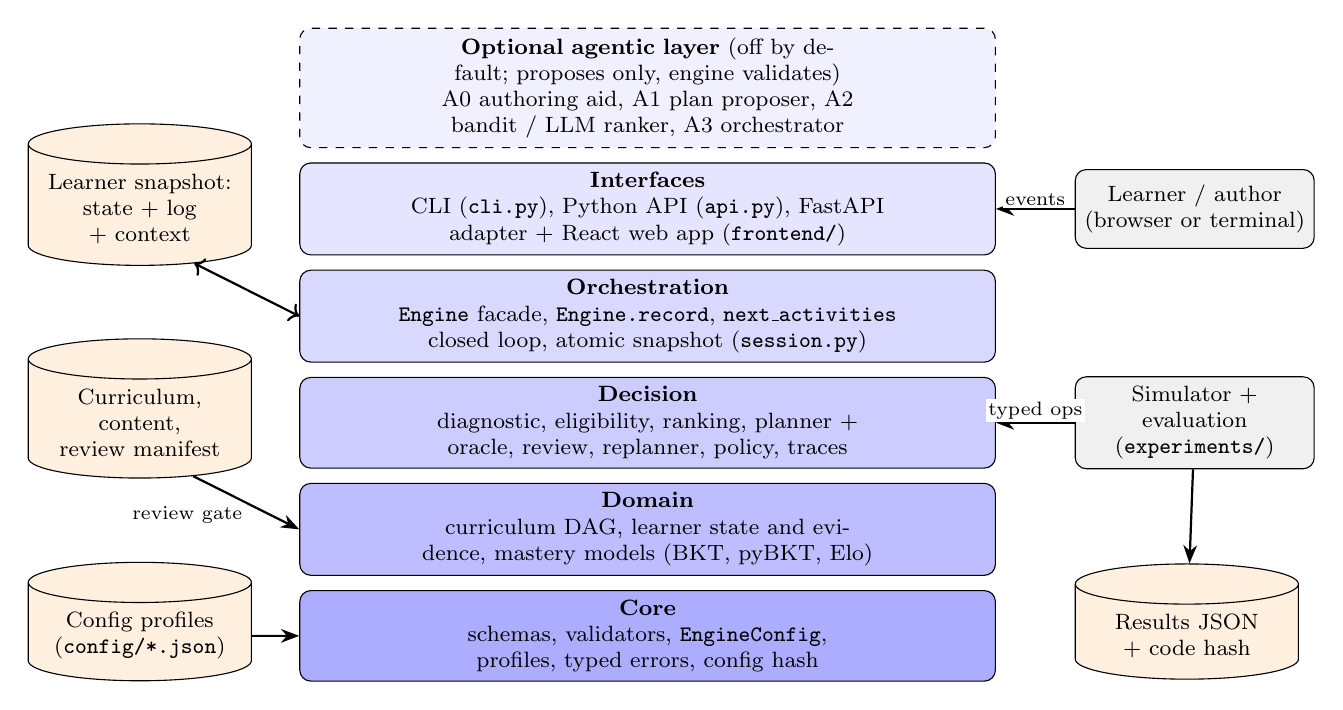
\begin{tikzpicture}[
  layer/.style={draw,rounded corners,text width=8.6cm,minimum height=1.0cm,align=center,font=\footnotesize},
  side/.style={draw,rounded corners,fill=gray!12,text width=2.8cm,minimum height=1.0cm,align=center,font=\footnotesize},
  store/.style={draw,cylinder,shape border rotate=90,aspect=0.18,fill=orange!12,text width=2.6cm,minimum height=1.0cm,align=center,font=\footnotesize},
  arr/.style={-{Stealth},thick},
  lab/.style={font=\scriptsize,fill=white,inner sep=1pt},
  node distance=0.18cm]
\node[layer,fill=blue!6,dashed] (L0) {\textbf{Optional agentic layer} (off by default; proposes only, engine validates)\\A0 authoring aid, A1 plan proposer, A2 bandit / LLM ranker, A3 orchestrator};
\node[layer,fill=blue!10,below=of L0] (L1) {\textbf{Interfaces}\\CLI (\texttt{cli.py}), Python API (\texttt{api.py}), FastAPI adapter + React web app (\texttt{frontend/})};
\node[layer,fill=blue!15,below=of L1] (L2) {\textbf{Orchestration}\\\texttt{Engine} facade, \texttt{Engine.record}, \texttt{next\_activities} closed loop, atomic snapshot (\texttt{session.py})};
\node[layer,fill=blue!20,below=of L2] (L3) {\textbf{Decision}\\diagnostic, eligibility, ranking, planner + oracle, review, replanner, policy, traces};
\node[layer,fill=blue!26,below=of L3] (L4) {\textbf{Domain}\\curriculum DAG, learner state and evidence, mastery models (BKT, pyBKT, Elo)};
\node[layer,fill=blue!32,below=of L4] (L5) {\textbf{Core}\\schemas, validators, \texttt{EngineConfig}, profiles, typed errors, config hash};
\node[side,right=1.0cm of L1] (ui) {Learner / author\\(browser or terminal)};
\node[side,right=1.0cm of L3] (sim) {Simulator + evaluation\\(\texttt{experiments/})};
\node[store,left=0.6cm of L3] (cur) {Curriculum, content,\\review manifest};
\node[store,left=0.6cm of L1] (snap) {Learner snapshot:\\state + log + context};
\node[store,left=0.6cm of L5] (cfg) {Config profiles\\(\texttt{config/*.json})};
\node[store,right=1.0cm of L5] (res) {Results JSON\\+ code hash};
\draw[arr] (ui) -- node[lab,above]{events} (L1);
\draw[arr] (sim) -- node[lab,above]{typed ops} (L3);
\draw[arr] (cur.south east) -- node[lab,below left]{review gate} (L4.west);
\draw[arr,<->] (snap.south east) -- (L2.west);
\draw[arr] (cfg) -- (L5);
\draw[arr] (sim) -- (res);
\end{tikzpicture}}
\caption{Delivered components and data flow. Solid arrows are the default path; the dashed layer is optional and can only propose.}
\label{fig:arch}
\end{figure}

\subsection{Major components and interfaces}

\begin{xltabular}{\textwidth}{
    @{}
    >{\raggedright\arraybackslash}p{0.2\textwidth}
    >{\raggedright\arraybackslash}X
    >{\raggedright\arraybackslash}p{0.26\textwidth}
    @{}
}
\caption{Major components, their responsibilities and source folders.}
\label{tab:components}\\
\toprule
\textbf{Component} & \textbf{Responsibility and interface} & \textbf{Source} \\
\midrule
\endfirsthead
\toprule
\textbf{Component} & \textbf{Responsibility and interface} & \textbf{Source} \\
\midrule
\endhead
\bottomrule
\endfoot
Core & Typed dataclasses, strict validators, \texttt{EngineConfig}, named profiles (\texttt{load\_profile}, \texttt{PRODUCT\_OVERRIDES}), typed errors, SHA-256 config hash. & \repodir{src/adaptengine/core} \\
Curriculum & \texttt{load\_curriculum}, \texttt{load\_activities}, \texttt{load\_content}; rejects unknown prerequisites and cycles; checks the review manifest. & \repodir{src/adaptengine/curriculum} \\
Learner & Immutable state, evidence fields, attempt-ID idempotency, \texttt{MasteryModel} protocol with \texttt{CustomBKT}, \texttt{PyBKTAdapter} and \texttt{EloModel}. & \repodir{src/adaptengine/learner} \\
Diagnostic & EIG item selection, entropy stop, caps, goal-path scope, prerequisite inference (\texttt{INFERRED}), optional state-space diagnostic. & \repodir{src/adaptengine/diagnostic} \\
Planner & Workload projection, hard filter, ranking, day packing, feasibility bounds, branch-and-bound oracle, best-effort plans, optional CP-SAT, proposal validation. & \repodir{src/adaptengine/planner} \\
Review & Half-life recall $r(t)=2^{-\Delta t/h}$, urgency, remediation, optional HLR-lite. & \repodir{src/adaptengine/review} \\
Replanner & Folds deadline and budget events into the context; full or frontier (memoised) replanning. & \repodir{src/adaptengine/replanner} \\
Policy & \texttt{DeterministicPolicy}; LinUCB bandit with logged propensities; LLM ranker with fallback. & \repodir{src/adaptengine/policy} \\
Agents, authoring & Plan proposer, orchestrator; draft generation with authoring checks and providers. & \repodir{src/adaptengine/agents}, \repodir{src/adaptengine/authoring} \\
Orchestration & \texttt{Engine.record(state, log, event)} as the only mutation boundary; atomic snapshot (\texttt{tmp} $\rightarrow$ \texttt{fsync} $\rightarrow$ \texttt{os.replace}). & \repo{src/adaptengine/api.py}, \repo{src/adaptengine/session.py} \\
Web adapter and app & 11 screens (setup, diagnostic, map, plan + Why?, study, disruptions, autopilot, evaluation, policy lab, authoring studio, overview). No decision logic: API plans equal direct engine calls. & \repodir{frontend/api}, \repodir{frontend/web} \\
Simulator and harness & Worlds S0--S4, S4F; arms; paired bootstrap; Kaplan--Meier; OPE; pre-registered runners E1--E6. & \repodir{experiments}, \repo{scripts/run_experiments.py} \\
\end{xltabular}

\subsection{Data stores, APIs and dependencies}

\begin{itemize}
\item \textbf{Data stores} are JSON files only. Curriculum and activities live in \repodir{data/curriculum}, lesson and exercise text in \repodir{data/content}, and review hashes in \repo{data/review_manifest.json}. A learner snapshot holds state, log and context in one file. Schemas are described in \repo{docs/schema.md}.
\item \textbf{APIs.} The Python API is listed in \repo{docs/API_REFERENCE.md}. The HTTP API is described by \repo{frontend/web/openapi.json}, and its TypeScript types are generated from it.
\item \textbf{External dependencies.} The core needs only NetworkX. Optional extras are \texttt{[pybkt]}, \texttt{[solver]}, \texttt{[demo]}, \texttt{[agents]} and \texttt{[figures]}. The \texttt{[agents]} extra needs \texttt{ANTHROPIC\_API\_KEY} or a local Ollama model, and is never used by default.
\end{itemize}

\subsection{Security and trust boundaries}

\begin{itemize}
\item \textbf{Content boundary.} Live loaders accept content only if its SHA-256 hash is in the review manifest with a named human reviewer. A reviewer named ``AI'' or \texttt{PENDING} is rejected (D9, D54).
\item \textbf{Input boundary.} All validation happens before any change, so a rejected event leaves state and log unchanged. Correctness must be a real boolean, and event kinds are strict enums.
\item \textbf{Agent boundary.} Agent output is untrusted. The engine checks that every chosen ID was offered and fits the budget, and a proposal is checked against 8 rules. Any failure falls back to the deterministic path.
\item \textbf{Network boundary.} Core packages never import providers or network clients (architecture test). The web adapter binds to 127.0.0.1 and has no authentication; it is a local demo only.
\end{itemize}

\subsection{Major ADRs}

The full log is \repo{docs/DECISIONS.md} (D1--D63), with approvals in \repo{docs/FREEZE_RECORD.md}. The decisions that shaped the final system are D6 (difficulty classes), D31 (lessons versus evidence), D32 (atomic snapshot), D35 (frontier replanning), D41--D44 (closed loop, best effort, reachable review, diagnostic selection), D46 (executed-state safety audit), D47 (simulator worlds and pre-registration), D49--D52 (consolidation, probe, strictness, optional diagnostic), D53--D58 (agentic layer), and D61--D63 (product configuration).

%==================================================== 4
\section{Methodology and Experiment Setup}

\subsection{Evaluation questions}

\begin{enumerate}[label=Q\arabic*.]
\item Does the adaptive engine keep every hard constraint while the learner actually answers (executed state, not the plan)?
\item Does the shipped product configuration reach goal mastery more often than non-adaptive baselines, and where?
\item Which parts matter: diagnostic, spaced review, consolidation and replanning (ablations)?
\item Is the adaptive diagnostic more accurate than fixed and random selection at the same item count (TC2.1)?
\item How sensitive is the result to the heuristic parameters?
\item Do the bandit policy and the extensions (Elo, HLR, BKT forgetting, CP-SAT) help?
\item Is planning and replanning fast enough for interactive use?
\end{enumerate}

\subsection{Workload, worlds and provenance}

There is no real learner data. Learners come from a transparent simulator whose dynamics differ from the engine's BKT model (except in S4, which is used as the matched case):
\begin{itemize}
\item \textbf{S0}: true ability $\theta\sim U(0.10,0.90)$ per concept, 2PL response with $a=3.0$.
\item \textbf{S1}: S0 plus readiness gating $\text{sigmoid}(10(\theta_{\text{pre}}-0.70))$, so learning depends on prerequisites.
\item \textbf{S2}: correlated abilities; \textbf{S3}: per-learner forgetting with $h\sim U(5,30)$ days.
\item \textbf{S4}: the engine's own BKT heuristics; \textbf{S4F}: S4 with parameters fitted on ASSISTments 2009~\cite{feng2009}.
\end{itemize}
A concept is truly mastered when $\theta\ge0.70$. Curricula are \texttt{4node\_x10}, \texttt{8node\_x10}, \texttt{synth-20-x10} and \texttt{synth-50-x10}, each with 10 exercises per concept at difficulties $0.1,\dots,0.9$. Parameter sources are listed in \repo{docs/EVALUATION_PROTOCOL.md}.

\subsection{Product configuration under test}

\texttt{product\_config(profile)} uses $\theta=0.95$, $k=1$, consolidation off, verification probe on, goal-search diagnostic on the goal path, \texttt{concept\_cap} 4, $N_{\max}=25$, and the \texttt{fitted\_S1} learner profile in every world (D61--D63). The old Week~8 configuration is kept as the arm \texttt{w8\_final}.

\subsection{Protocol, seeds and statistics}

\begin{itemize}
\item \textbf{Pre-registration:} \repo{docs/preregistration/PRODUCT_RERUN_2026-11-15.md}, with one amendment made before any full run. The runner refuses to start if the source hash (\texttt{6c55d4f99dc1\ldots}) or the experiment hash (\texttt{24eabf602925\ldots}) differs.
\item \textbf{Seeds:} fitting and training use even seeds; reporting uses odd seeds only, 200 learners per cell and 1000 in the headline cell (S1, \texttt{4node\_x10}, 15 min/day, calm, 14 days).
\item \textbf{Grid (E1):} 4 worlds $\times$ 2 curricula $\times$ budgets \{10, 15\} $\times$ \{calm, missed\_day, missed\_2days\} $\times$ horizons \{W7 rule, 7, 14, 21 days\}, plus a forgetting scenario: 208 primary cells. A further 135 stress cells use budget and deadline shocks. In total, 462,600 episodes.
\item \textbf{Statistics:} paired bootstrap 95\% CI (2000 resamples, seed 20260), no multiplicity correction, every cell reported. A cell is ``better'' or ``worse'' only when its CI excludes 0.
\end{itemize}

\subsection{Environment and run scripts}

Runs used one laptop (Intel Core i7-1360P, 16 threads, 16\,GB RAM, Linux), Python 3.11.17, NetworkX 3.4.2 and OR-Tools for E6. The full grid took 5195\,s. Every result file records its code hash, experiment hash and UTC timestamp.

\begin{xltabular}{\textwidth}{
    @{}
    >{\raggedright\arraybackslash}p{0.12\textwidth}
    >{\raggedright\arraybackslash}X
    >{\raggedright\arraybackslash}p{0.3\textwidth}
    @{}
}
\caption{Experiment scripts. \texttt{make final} runs all of them in order and then builds \protect\repo{docs/RESULTS.md}.}
\label{tab:scripts}\\
\toprule
\textbf{ID} & \textbf{Command} & \textbf{Output} \\
\midrule
\endfirsthead
\toprule
\textbf{ID} & \textbf{Command} & \textbf{Output} \\
\midrule
\endhead
\bottomrule
\endfoot
E1 & \texttt{python experiments/run\_grid.py --grid both} & \texttt{grid.json} \\
E2 & \texttt{python experiments/run\_diag.py} & \texttt{diag\_matrix.json} \\
E3 & \texttt{python experiments/run\_sensitivity.py} & \texttt{sensitivity.json} \\
E4 & \texttt{python experiments/run\_policy.py train}, then \texttt{eval} & \texttt{policy\_eval.json} \\
E5 & \texttt{python experiments/run\_extensions.py all} & \texttt{extensions.json} \\
E6 & \texttt{python experiments/run\_planner\_cost.py all} & \texttt{planner\_cost.json} \\
All & \texttt{make final} (\texttt{scripts/run\_experiments.py}) & \texttt{experiments/results/}, \texttt{docs/RESULTS.md} \\
\end{xltabular}

%==================================================== 5
\section{Results, Observations and Analysis}

All numbers below are copied from \repo{docs/RESULTS.md}, which is generated from the result files without hand editing. Rates are fractions of simulated learners (0--1); times are minutes of study or milliseconds of computation.

\subsection{Safety (Q1)}

\begin{xltabular}{\textwidth}{
    @{}
    >{\raggedright\arraybackslash}p{0.22\textwidth}
    >{\raggedright\arraybackslash}p{0.1\textwidth}
    >{\raggedright\arraybackslash}p{0.08\textwidth}
    >{\raggedleft\arraybackslash}X
    >{\raggedleft\arraybackslash}X
    >{\raggedleft\arraybackslash}X
    @{}
}
\caption{Violations summed over all E1 cells.}
\label{tab:violations}\\
\toprule
\textbf{Arm} & \textbf{Adaptive} & \textbf{Cells} & \textbf{Executed prereq.} & \textbf{Plan prereq.} & \textbf{Budget} \\
\midrule
\endfirsthead
\toprule
\textbf{Arm} & \textbf{Adaptive} & \textbf{Cells} & \textbf{Executed prereq.} & \textbf{Plan prereq.} & \textbf{Budget} \\
\midrule
\endhead
\bottomrule
\endfoot
product & yes & 343 & 0 & 0 & 0 \\
product\_nodx, \_norev, \_consol & yes & 208 each & 0 & 0 & 0 \\
w8\_final & yes & 208 & 0 & 0 & 0 \\
random\_eligible & no & 208 & 0 & 0 & 0 \\
product\_noreplan & no & 343 & 1,034,357 & 193,600 & 9,000 \\
static & no & 208 & 1,118,764 & 289,600 & 0 \\
static\_loop & no & 343 & 1,660,407 & 338,200 & 0 \\
\end{xltabular}

Every adaptive arm also had 0 violations in E3 (31 configurations), E4 (4 policy variants, 800 training episodes) and E5 (all extensions). The non-adaptive baselines reach the goal partly by studying concepts whose prerequisites are not mastered. The open-loop plan also overruns the budget after disruptions. \textbf{Q1 is met.}

\subsection{Headline cell (Q2)}

\begin{xltabular}{\textwidth}{
    @{}
    >{\raggedright\arraybackslash}p{0.17\textwidth}
    >{\raggedleft\arraybackslash}X
    >{\raggedleft\arraybackslash}X
    >{\raggedleft\arraybackslash}X
    >{\raggedleft\arraybackslash}X
    >{\raggedleft\arraybackslash}X
    >{\raggedleft\arraybackslash}p{0.27\textwidth}
    @{}
}
\caption{Baseline comparison, headline cell S1 $|$ \texttt{4node\_x10} $|$ 15 min/day $|$ calm $|$ 14 days, $N=1000$ paired learners. Goal, all-required and false mastery are rates; utilisation is the share of available minutes used; KM median is minutes to goal mastery (--- if not reached).}
\label{tab:headline}\\
\toprule
\textbf{Arm} & \textbf{Goal} & \textbf{All req.} & \textbf{False mast.} & \textbf{Util.} & \textbf{KM med.} & \textbf{$\Delta$ goal vs static\_loop [95\% CI]} \\
\midrule
\endfirsthead
\toprule
\textbf{Arm} & \textbf{Goal} & \textbf{All req.} & \textbf{False mast.} & \textbf{Util.} & \textbf{KM med.} & \textbf{$\Delta$ goal vs static\_loop [95\% CI]} \\
\midrule
\endhead
\bottomrule
\endfoot
\textbf{product} & \textbf{0.792} & 0.562 & 0.152 & 0.64 & 119 & +0.032 [+0.003, +0.061] \\
product\_nodx & 0.808 & 0.619 & 0.130 & 0.58 & 105 & +0.048 [+0.020, +0.076] \\
product\_consol & 0.938 & 0.874 & 0.038 & 0.95 & 119 & +0.178 [+0.154, +0.203] \\
product\_norev & 0.810 & 0.618 & 0.130 & 0.58 & 105 & +0.050 [+0.021, +0.078] \\
product\_noreplan & 0.349 & 0.060 & 0.189 & 0.28 & --- & $-$0.411 [$-$0.441, $-$0.381] \\
w8\_final & 0.927 & 0.869 & 0.043 & 0.95 & 107 & +0.167 [+0.144, +0.191] \\
static\_loop & 0.760 & 0.709 & 0.011 & 0.99 & 134 & --- \\
static & 0.399 & 0.101 & 0.097 & 0.37 & --- & $-$0.361 [$-$0.391, $-$0.332] \\
random\_eligible & 0.384 & 0.367 & 0.002 & 1.00 & --- & $-$0.376 [$-$0.405, $-$0.346] \\
\end{xltabular}

\begin{figure}[H]
\centering
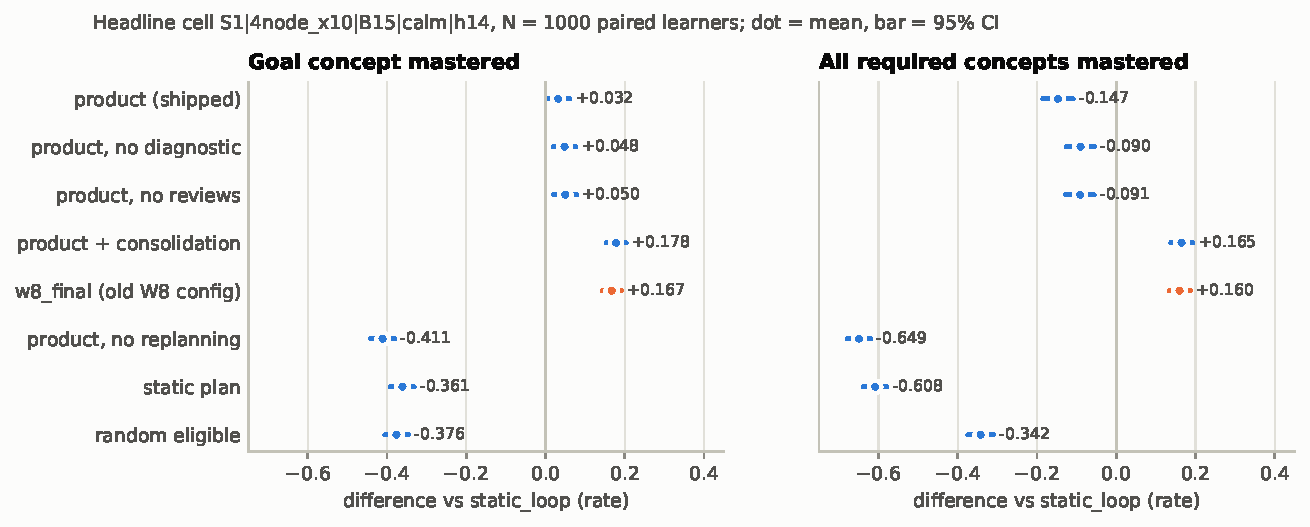
\includegraphics[width=\textwidth]{fig2_headline_paired_differences}
\caption{Paired differences against \texttt{static\_loop} in the headline cell. Source: \texttt{grid.json}.}
\label{fig:headline}
\end{figure}

In the headline cell the product engine reaches the goal slightly more often than \texttt{static\_loop} ($+0.032$) and faster (KM median 119 versus 134 minutes). However, it masters \emph{all} required concepts less often ($-0.147$) and has more false mastery (0.152 versus 0.011). The reason is visible in utilisation: with consolidation off, the product engine stops at about 64\% of the available minutes once it believes the goal is mastered. Turning consolidation on (\texttt{product\_consol}) or using the Week~8 configuration gives the best results in this cell.

\subsection{Across the grid (Q2)}

\begin{figure}[H]
\centering
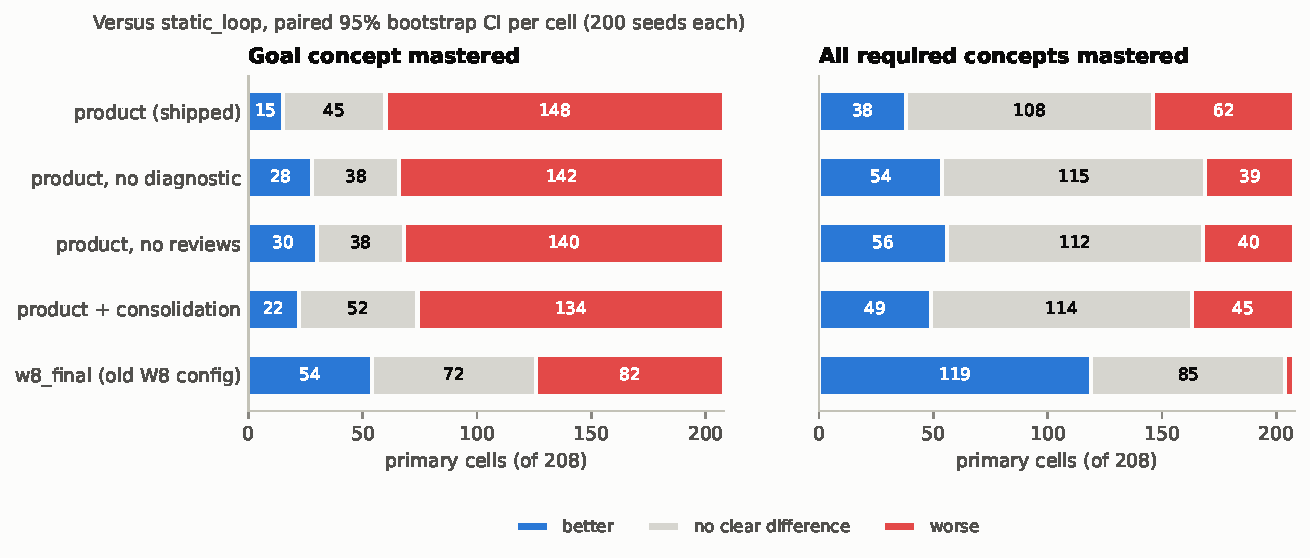
\includegraphics[width=\textwidth]{fig1_win_tie_loss_vs_static_loop}
\caption{Cells where each arm is better, not clearly different or worse than \texttt{static\_loop} (208 primary cells, paired 95\% CI). Source: \texttt{grid.json}.}
\label{fig:wintieloss}
\end{figure}

\begin{xltabular}{\textwidth}{
    @{}
    >{\raggedright\arraybackslash}X
    >{\raggedleft\arraybackslash}p{0.12\textwidth}
    >{\raggedleft\arraybackslash}p{0.12\textwidth}
    >{\raggedleft\arraybackslash}p{0.12\textwidth}
    >{\raggedleft\arraybackslash}p{0.14\textwidth}
    @{}
}
\caption{Product versus \texttt{static\_loop} on goal mastery by horizon (cells by 95\% CI).}
\label{tab:horizon}\\
\toprule
\textbf{Horizon} & \textbf{Better} & \textbf{n.s.} & \textbf{Worse} & \textbf{Mean $\Delta$} \\
\midrule
\endfirsthead
\toprule
\textbf{Horizon} & \textbf{Better} & \textbf{n.s.} & \textbf{Worse} & \textbf{Mean $\Delta$} \\
\midrule
\endhead
\bottomrule
\endfoot
W7 rule (short) & 0 & 0 & 48 & $-$0.076 \\
7 days & 0 & 2 & 46 & $-$0.105 \\
14 days & 5 & 13 & 30 & $-$0.075 \\
21 days (incl. forgetting) & 10 & 30 & 24 & $-$0.034 \\
\midrule
All 208 cells, goal mastery & 15 & 45 & 148 & --- \\
All 208 cells, all-required mastery & 38 & 108 & 62 & $-$0.012 \\
\end{xltabular}

\textbf{Observation.} The gain depends on the world and the horizon. The product engine is best in S1 (the prerequisite-gated world): for example, S1 \texttt{4node\_x10} at 14 days has a mean of $+0.082$, and S1 \texttt{8node\_x10} at 21 days $+0.059$. It is clearly worse in S4 \texttt{8node\_x10} ($-0.19$ to $-0.22$) and with short horizons. With little time, a state-blind loop that practises the goal from the first minute wins, because the engine spends minutes on the diagnostic and on prerequisites. \textbf{Q2 is only partly met:} the product is safe and better than static, random and open-loop plans, but not better than \texttt{static\_loop} in most cells.

\subsection{Ablations and comparison with Week 8 (Q3)}

\begin{xltabular}{\textwidth}{
    @{}
    >{\raggedright\arraybackslash}X
    >{\raggedleft\arraybackslash}p{0.17\textwidth}
    >{\raggedleft\arraybackslash}p{0.1\textwidth}
    >{\raggedleft\arraybackslash}p{0.17\textwidth}
    >{\raggedleft\arraybackslash}p{0.1\textwidth}
    @{}
}
\caption{Paired ablations over 208 primary cells (better / n.s. / worse by 95\% CI; mean is the unweighted mean of per-cell differences).}
\label{tab:ablations}\\
\toprule
\textbf{Comparison} & \textbf{Goal B/N/W} & \textbf{Mean} & \textbf{All-req. B/N/W} & \textbf{Mean} \\
\midrule
\endfirsthead
\toprule
\textbf{Comparison} & \textbf{Goal B/N/W} & \textbf{Mean} & \textbf{All-req. B/N/W} & \textbf{Mean} \\
\midrule
\endhead
\bottomrule
\endfoot
Diagnostic: product $-$ product\_nodx & 2 / 152 / 54 & $-$0.018 & 0 / 118 / 90 & $-$0.036 \\
Consolidation: product\_consol $-$ product & 34 / 174 / 0 & +0.016 & 39 / 169 / 0 & +0.040 \\
Review: product $-$ product\_norev & 0 / 147 / 61 & $-$0.021 & 0 / 115 / 93 & $-$0.037 \\
Replanning: product $-$ product\_noreplan & 60 / 74 / 74 & +0.011 & 119 / 75 / 14 & +0.197 \\
Product $-$ w8\_final & 0 / 85 / 123 & $-$0.068 & 0 / 67 / 141 & $-$0.119 \\
\end{xltabular}

\begin{itemize}
\item \textbf{Replanning} is the most valuable part for full mastery ($+0.197$ all-required). On goal-only mastery it is mixed, because the open-loop plan studies the goal early, with violations.
\item \textbf{Consolidation} never made a cell worse and helped in 34. It is off in the product only by an owner decision (D63).
\item \textbf{The diagnostic and spaced review cost study minutes} and do not pay back within 7--21 days. They are worse in 54 and 61 cells respectively.
\item \textbf{The product is never better than the old Week~8 configuration} (0 cells better, 123 worse on goal). The stricter mastery rule ($\theta=0.95$, D61) and consolidation off explain most of the gap (see also sensitivity). This is a regression that is disclosed and recorded in the backlog.
\end{itemize}

\subsection{Diagnostic accuracy (Q4, TC2.1)}

\begin{xltabular}{\textwidth}{
    @{}
    >{\raggedright\arraybackslash}X
    >{\raggedleft\arraybackslash}p{0.14\textwidth}
    >{\raggedleft\arraybackslash}p{0.14\textwidth}
    >{\raggedleft\arraybackslash}p{0.14\textwidth}
    >{\raggedleft\arraybackslash}p{0.14\textwidth}
    @{}
}
\caption{Day-0 diagnostic accuracy against truth $\mathbb{1}[\theta\ge0.70]$, mean over 16 cells (4 worlds $\times$ 4 curricula, 200 learners each). Higher AUC and lower Brier are better.}
\label{tab:diag}\\
\toprule
\textbf{Arm} & \textbf{AUC} & \textbf{Brier} & \textbf{MAE} & \textbf{Items} \\
\midrule
\endfirsthead
\toprule
\textbf{Arm} & \textbf{AUC} & \textbf{Brier} & \textbf{MAE} & \textbf{Items} \\
\midrule
\endhead
\bottomrule
\endfoot
Prior only & 0.500 & 0.174 & 0.298 & 0 \\
\textbf{Product (goal path)} & \textbf{0.667} & \textbf{0.175} & \textbf{0.277} & \textbf{14.4} \\
Product (all concepts) & 0.664 & 0.175 & 0.278 & 15.3 \\
Week 7 concept sweep & 0.586 & 0.167 & 0.289 & 4.3 \\
Frontier & 0.604 & 0.164 & 0.287 & 7.7 \\
fixed@n (same items) & 0.705 & 0.155 & 0.275 & 15.3 \\
random@n (same items) & 0.681 & 0.159 & 0.279 & 15.3 \\
irt\_cat@n (true $a$) & 0.627 & 0.199 & 0.313 & 15.3 \\
\end{xltabular}

The product diagnostic ranks learners much better than the prior (AUC 0.667 versus 0.500) and better than the Week~7 diagnostic. It is still \emph{worse} than fixed-order and random selection at the same item count on both AUC and Brier, and its Brier score equals the prior. \textbf{The TC2.1 error clause is not met.} The likely cause is that EIG concentrates items on a few concepts and on hard items (noted in the mid report), while fixed order spreads them. Each diagnostic takes 0.9--3.7\,ms to compute.

\subsection{Sensitivity (Q5)}

\begin{figure}[H]
\centering
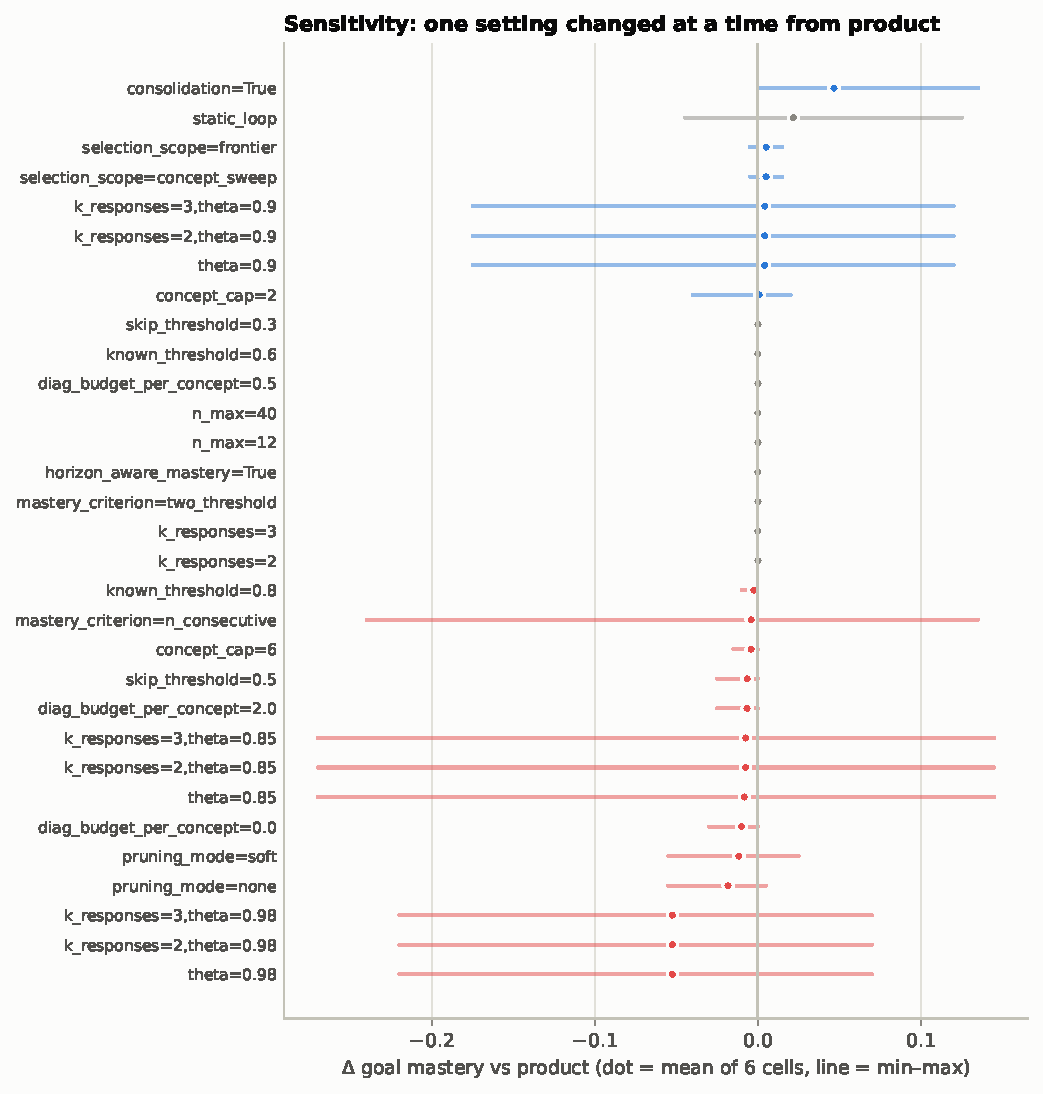
\includegraphics[width=0.9\textwidth]{fig6_sensitivity}
\caption{One-at-a-time sensitivity around the product configuration (S0, S1, S4 $\times$ 2 curricula, 15 min/day, 14 days). Source: \texttt{sensitivity.json}.}
\label{fig:sens}
\end{figure}

Most settings have no effect ($k$, $N_{\max}$, horizon-aware strictness, known threshold, selection scope). Consolidation on is better in 4 of 6 cells (mean $+0.047$). $\theta=0.98$ is worse in 4 of 6 cells (mean $-0.052$). Lowering $\theta$ to 0.85 or 0.90 is better in 3 cells and worse in 2, so the result depends on the world. Removing pruning is worse in 2 cells. Every configuration had 0 violations.

\subsection{Policy, extensions and planner cost (Q6, Q7)}
\label{sec:extensions}

\begin{itemize}
\item \textbf{LinUCB bandit (E4).} Frozen, updating and random rankings matched the deterministic ranking in 3 of 4 cells. In S1 \texttt{8node\_x10}, frozen and updating were $+0.020$ [$+0.005$, $+0.040$], and random was $+0.020$ [0.000, $+0.045$]. Since random does as well, ranking order matters little here. Off-policy estimates of the frozen policy were within 0.011 of its simulated value from random logs and within 0.001 from updating logs.
\item \textbf{Elo/1PL (D59)} lowered goal mastery by 0.515--0.650. \textbf{BKT with forgetting} lowered it by 0.490, since $\theta=0.95$ becomes unreachable. \textbf{HLR-lite} fitted worse than a constant rate (Brier 0.302 versus 0.245) and was mixed in use ($+0.040$ on 4 nodes, $-0.150$ on 8 nodes). The \textbf{review cap} had no measurable effect, because no arm reached the goal on \texttt{synth-20-x10} under fast forgetting. All extensions stay off by default.
\item \textbf{CP-SAT (D60).} On \texttt{synth-20-x10} with a 21-day deadline, CP-SAT used 289 instead of 307 minutes and removed 9 duplicate reviews. However, it took 5033\,ms instead of 9.8\,ms. On \texttt{synth-50-x10} it hit its 5\,s limit and fell back. Both planners had 0 violations, and both returned the same \texttt{INFEASIBLE} verdict at tight deadlines.
\item \textbf{Latency.} Initial planning takes 1.9--37.6\,ms. Frontier replanning gives the same plans as full recomputation in 16 of 16 cases and is 1.14--1.48$\times$ faster (\texttt{synth-50-x10}: 28.7 versus 35.4\,ms for a missed day). \textbf{Q7 is met.}
\end{itemize}

\subsection{Greedy versus CP-SAT on tight deadlines (exploratory)}
\label{sec:cpsat}

E6 sets its deadlines from the greedy plan itself (100\%, 90\% and 80\% of its length), so it rarely tests the cases where the two planners can disagree. This separate experiment targets those cases. It was \textbf{not pre-registered}. It ran on source hash \texttt{fabcac29\ldots}, which includes one engine fix: when CP-SAT proves that no packing exists, the engine now returns \texttt{INFEASIBLE} (\texttt{CPSAT\_INFEASIBLE}) instead of discarding the proof and returning \texttt{UNKNOWN}. The experiment hash is unchanged. Script: \repo{scripts/cpsat_vs_greedy.py}; results: \repo{experiments/results/cpsat_vs_greedy.json} (922\,s).

\textbf{Setup.} Both arms use the product engine (\texttt{fitted\_S1}) with maintenance reviews off:
\begin{itemize}
\item \textbf{greedy} is greedy packing; when greedy misses the deadline it falls back to the branch-and-bound oracle (node limit 1000).
\item \textbf{CP-SAT} is exact packing with a 5\,s limit; if CP-SAT cannot decide, it falls back to greedy.
\item \textbf{hybrid} is what the web app runs: greedy first, then CP-SAT only when greedy returns \texttt{UNKNOWN}. Its results are derived from the other two arms.
\end{itemize}
A case is a curriculum, a goal, a daily budget (5, 10, 15 or 30 minutes) and a learner state (fresh, or one of 3 seeded partly-known states). $L$ is the last day of the greedy plan when the deadline is far away. For each case, the deadlines run from $L$ downwards. They stop at the first deadline that both arms reject by the time-budget bound alone, so only deadlines that need real packing are kept. Each arm was timed once per instance after a warm-up. CP-SAT's own verdict was recorded separately, because a CP-SAT timeout falls back to greedy.

\begin{xltabular}{\textwidth}{
    @{}
    >{\raggedright\arraybackslash}X
    >{\raggedleft\arraybackslash}p{0.17\textwidth}
    >{\raggedleft\arraybackslash}p{0.17\textwidth}
    >{\raggedleft\arraybackslash}p{0.17\textwidth}
    @{}
}
\caption{Greedy (+ oracle) versus CP-SAT on deadlines between the time-budget bound and the greedy plan length. Latency is median / p95 / max in milliseconds.}
\label{tab:cpsat}\\
\toprule
\textbf{Measure} & \textbf{4node\_x10} & \textbf{8node\_x10} & \textbf{synth-20-x10} \\
\midrule
\endfirsthead
\toprule
\textbf{Measure} & \textbf{4node\_x10} & \textbf{8node\_x10} & \textbf{synth-20-x10} \\
\midrule
\endhead
\bottomrule
\endfoot
Instances (cases) & 72 (64) & 142 (120) & 270 (64) \\
Greedy \texttt{UNKNOWN} & 8 & 18 & 74 \\
CP-SAT \texttt{UNKNOWN} & 0 & 0 & 35 \\
Greedy \texttt{UNKNOWN}, CP-SAT finds a plan & 3 & 8 & 24 \\
Greedy \texttt{UNKNOWN}, CP-SAT proves \texttt{INFEASIBLE} & 5 & 10 & 15 \\
Greedy feasible, CP-SAT not & 0 & 0 & 0 \\
Cases with a shorter feasible deadline under CP-SAT & 3 of 64 & 8 of 120 & 18 of 64 \\
Days saved on the shortest feasible deadline (mean / max) & 0.05 / 1 & 0.07 / 1 & 0.45 / 4 \\
Mean last plan day when both are feasible & 3.22 vs 3.17 & 4.36 vs 4.25 & 48.20 vs 47.77 \\
Greedy latency & 2.1 / 6.7 / 8.1 & 2.4 / 8.6 / 14.5 & 14.2 / 35.3 / 58.1 \\
CP-SAT latency & 5.5 / 59.2 / 188.9 & 7.7 / 196.1 / 1037.7 & 5058 / 5263 / 5322 \\
Hybrid latency & 2.1 / 40.4 / 105.1 & 2.4 / 50.6 / 731.5 & 19.1 / 5139 / 5309 \\
\end{xltabular}

\textbf{Observations.}
\begin{itemize}
\item \textbf{CP-SAT plans better.} Over all 484 instances, greedy could not decide 100 (21\%) and CP-SAT 35 (7\%). In 35 instances CP-SAT found a plan where greedy returned \texttt{UNKNOWN}. In 30 more it proved that no plan exists. It never lost a plan that greedy had found. It also reached the goal earlier: in 29 of 248 cases its shortest feasible deadline was 1--4 days shorter.
\item \textbf{CP-SAT costs time, and the cost grows with size.} On the 4- and 8-concept curricula CP-SAT took 2--3$\times$ the median greedy time and up to about 1\,s. On \texttt{synth-20-x10} it hit its 5\,s limit in 142 of 270 instances (median 5.06\,s against 14\,ms for greedy). All 35 of its remaining \texttt{UNKNOWN} results are on this curriculum.
\item \textbf{The hybrid keeps most of the benefit.} The hybrid has the same outcomes as CP-SAT with greedy's median latency, because CP-SAT runs only when greedy is undecided. The cost is in the tail: up to 5.3\,s for those replans.
\item \textbf{Safety.} \texttt{validate\_proposal} found no prerequisite, budget, deadline or duplicate violation in any feasible plan of either arm. One instance (\texttt{synth-20-x10}, goal C20, 5\,min/day, fresh learner) failed the goal-reached rule in both arms. The plan comes from greedy, which CP-SAT fell back to after a timeout. It is a greedy defect: at 5\,min/day, due reviews take part of every day, a 4-minute lesson never fits, greedy stops after 15 days without progress, and the planner still reports \texttt{FEASIBLE} because the last planned day is before the deadline.
\end{itemize}

\subsection{Critical failure and edge cases}

\begin{xltabular}{\textwidth}{
    @{}
    >{\raggedright\arraybackslash}p{0.3\textwidth}
    >{\raggedright\arraybackslash}X
    >{\raggedright\arraybackslash}p{0.25\textwidth}
    @{}
}
\caption{Agreed failure and edge cases.}
\label{tab:edge}\\
\toprule
\textbf{Case} & \textbf{Observed} & \textbf{Evidence} \\
\midrule
\endfirsthead
\toprule
\textbf{Case} & \textbf{Observed} & \textbf{Evidence} \\
\midrule
\endhead
\bottomrule
\endfoot
Cycle or unknown prerequisite & Typed error naming the concepts; no change to state or log. & TC1.1, TC1.2 \\
Unreviewed or AI-signed content & Rejected by every live loader. & \repo{tests/test_loader_review_gate.py} \\
Goal cannot fit before deadline & \texttt{INFEASIBLE} with shortfall, options and a best-effort plan. & TC3.4 \\
Bounds pass but packing fails ($8+8+4$, 10 min) & Oracle returns \texttt{INFEASIBLE}. & TC3.5 \\
Oracle node limit & \texttt{UNKNOWN}, never a false \texttt{INFEASIBLE}. & TC3.6 \\
Budget crash 30$\rightarrow$5, deadline halved & 0 violations; goal mastery drops with available time (stress grid, 135 cells). & \texttt{grid.json} \\
Interrupted save & Fault injection on \texttt{os.replace}: no partial file, state unchanged. & \repo{tests/test_feedback_fixes.py} \\
Adversarial agent output & Falls back to deterministic plan with 0 violations. & \repo{tests/test_agent_policy.py} \\
Replayed \texttt{attempt\_id} & Ignored; mastery not inflated. & \repo{tests/test_feedback_fixes.py} \\
\end{xltabular}

\subsection{Tests not run}

\begin{itemize}
\item Live LLM agents (A0 authoring aid with a real model, A1, A2$'$, A3) were \textbf{not evaluated with a model}. Only stub-provider plumbing tests ran.
\item No real-learner data, pilot or Python-specific dataset (CSEDM, Junyi) was used.
\item Consolidation and the verification probe were not separated in any run.
\item E2 (diagnostic) was not run on S3 or S4F; E4 ran only S1 and S4.
\end{itemize}

%==================================================== 6
\section{Milestone Verification Matrix}

Test names are in \repo{docs/TRACEABILITY.md}; all files are under \repodir{tests}. The full suite has 444 tests. On 15 November 2026 (\texttt{pytest --cov=adaptengine}): \textbf{442 passed, 2 failed}, statement coverage 92\%. Both failures are in experiment-harness tests, not acceptance tests (Table~\ref{tab:risks}).

\begin{xltabular}{\textwidth}{
    @{}
    >{\raggedright\arraybackslash}p{0.07\textwidth}
    >{\raggedright\arraybackslash}p{0.08\textwidth}
    >{\raggedright\arraybackslash}X
    >{\raggedright\arraybackslash}X
    >{\raggedright\arraybackslash}p{0.08\textwidth}
    >{\raggedright\arraybackslash}p{0.21\textwidth}
    @{}
}
\caption{Frozen acceptance tests: expected versus observed.}
\label{tab:matrix}\\
\toprule
\textbf{MS} & \textbf{Test} & \textbf{Expected} & \textbf{Observed} & \textbf{Status} & \textbf{Evidence} \\
\midrule
\endfirsthead
\toprule
\textbf{MS} & \textbf{Test} & \textbf{Expected} & \textbf{Observed} & \textbf{Status} & \textbf{Evidence} \\
\midrule
\endhead
\bottomrule
\endfoot
M1 & TC1.1 & Cycle rejected with typed error. & \texttt{CycleError} naming concepts. & Pass & \texttt{test\_graph.py} \\
M1 & TC1.2 & Invalid or unreviewed input rejected, no change. & Rejected before any update. & Pass & \texttt{test\_schema.py}, \texttt{test\_loader\_} \texttt{review\_gate.py} \\
M2 & TC2.1 & Stops at threshold or cap; error no worse than fixed and random at equal budget. & Cap and stop hold. Error worse than fixed@n and random@n (Table~\ref{tab:diag}). & \textbf{Partial} (accuracy Fail) & \texttt{test\_diagnostic.py}, \texttt{diag\_matrix.json} \\
M2 & TC2.2 & Prior kept, \texttt{UNASSESSED}. & As expected. & Pass & \texttt{test\_diagnostic.py} \\
M2 & TC2.3 & Two learners get different valid plans. & Different, both valid. & Pass & \texttt{test\_planner.py} \\
M3 & TC3.1 & Locked concept never scheduled. & 0 plan and 0 executed violations. & Pass & \texttt{test\_planner.py}, \texttt{test\_arms.py} \\
M3 & TC3.2 & No day over budget. & 0 budget violations, including mid-day replans. & Pass & \texttt{test\_planner.py} \\
M3 & TC3.3 & 5 vs 30 min give different pacing. & Different number of days. & Pass & \texttt{test\_planner.py} \\
M3 & TC3.4 & \texttt{INFEASIBLE} + shortfall + options. & As expected, plus best effort. & Pass & \texttt{test\_planner.py}, \texttt{test\_w7\_planner.py} \\
M3 & TC3.5 & $8+8+4$: oracle \texttt{INFEASIBLE}. & As expected. & Pass & \texttt{test\_planner.py} \\
M3 & TC3.6 & Limit gives \texttt{UNKNOWN}. & As expected. & Pass & \texttt{test\_planner.py} \\
M4 & TC4.1 & 0.1707 and 0.2122; adapter = library. & Match; pyBKT parity at $10^{-9}$. & Pass & \texttt{test\_mastery.py}, \texttt{test\_adapter.py} \\
M4 & TC4.2 & Exercise nearest $P_c=0.75$, tie rule. & As expected. & Pass & \texttt{test\_planner.py} \\
M5 & TC5.1 & Mastered concept omitted, trace cites evidence. & As expected. & Pass & \texttt{test\_w5.py} \\
M5 & TC5.2 & $p<0.40$ inserts remediation. & Lesson inserted, flag set. & Pass & \texttt{test\_w5.py} \\
M5 & TC5.3 & Urgent review before new content. & As expected. & Pass & \texttt{test\_w5.py}, \texttt{test\_review.py} \\
M6 & TC6.1 & Missed day: valid plan, no loss. & As expected. & Pass & \texttt{test\_w5.py} \\
M6 & TC6.2 & Failed assessment: remediation plan. & As expected. & Pass & \texttt{test\_w5.py} \\
M6 & TC6.3 & Deadline change: plan or \texttt{INFEASIBLE}. & As expected. & Pass & \texttt{test\_w5.py} \\
M6 & TC6.4 & Budget change: plan within new budget. & As expected. & Pass & \texttt{test\_w5.py} \\
M7 & TC7.1 & Every decision traceable. & Exactly one \texttt{SELECTED} per activity. & Pass & \texttt{test\_w5.py}, \texttt{test\_planner.py} \\
M8 & TC8.1 & Identical seeds give identical results. & Bitwise identical. & Pass & \texttt{test\_evaluation.py}, \texttt{test\_arms.py} \\
M8 & TC8.2 & Frontier = full replanning; latency recorded. & 16/16 equal; 1.14--1.48$\times$ faster. & Pass & \texttt{test\_replan\_} \texttt{frontier.py}, \texttt{planner\_cost.json} \\
\end{xltabular}

\paragraph{Approved changes, flagged separately.} (i) TC2.1: the error metric changed from MAE to Brier and AUC against binary truth in Week~7 (D44), because MAE is not a proper score for a probability. (ii) TC3.1: the primary audit changed from the plan to the executed state (D46), after the Week~6 plan audit hid 183 violations. (iii) $N_{\max}$ changed from 8 to 6 (D44) and then to 25 for the goal-search diagnostic (D62). (iv) The product configuration (D61--D63) overrides the Week~8 selection. Approval for (iii) and (iv): \fillin{mentor approval reference, if any}.

%==================================================== 7
\section{Mentor Feedback and Engineering Evolution}

\subsection{Feedback closure}

\begin{xltabular}{\textwidth}{
    @{}
    >{\raggedright\arraybackslash}p{0.11\textwidth}
    >{\raggedright\arraybackslash}p{0.22\textwidth}
    >{\raggedright\arraybackslash}p{0.13\textwidth}
    >{\raggedright\arraybackslash}X
    >{\raggedright\arraybackslash}p{0.2\textwidth}
    @{}
}
\caption{Scored mentor feedback and the team response.}
\label{tab:feedback}\\
\toprule
\textbf{FB-ID} & \textbf{Mentor request} & \textbf{Status} & \textbf{Change} & \textbf{Evidence} \\
\midrule
\endfirsthead
\toprule
\textbf{FB-ID} & \textbf{Mentor request} & \textbf{Status} & \textbf{Change} & \textbf{Evidence} \\
\midrule
\endhead
\bottomrule
\endfoot
W2 review & Review gate bypassed by CLI; unchecked types; phantom prerequisite nodes; lessons set \texttt{assessed}; two-file save. & Implemented & Mandatory review gate, strict validators, reference checks before edges, evidence-state split, atomic snapshot. & \texttt{test\_loader\_} \texttt{review\_gate.py}, \texttt{test\_defects\_} \texttt{repro.py} \\
FB001 & Reuse an established model library. & Implemented & Real pyBKT 1.4.3 model behind \texttt{MasteryModel}; parity at $10^{-9}$. & \texttt{test\_feedback\_fixes.py} \\
FB002 & Uncertainty semantics, caps, one observation model, attempt IDs. & Implemented & EIG uses the injected model (D33); session-scoped IDs (D34); config-driven mastery. & \texttt{test\_feedback\_fixes.py} \\
FB003 & Stale decision and traceability records. & Implemented & D-log and 23-ID register synchronised; D19 marked reserved; W7 corrected test paths. & \repo{docs/DECISIONS.md}, \repo{docs/TRACEABILITY.md} \\
FB004 & \fillin{request text} & \fillin{status} & \fillin{change} & \fillin{evidence} \\
FB005 / W2-FB005 & Config ignored; permissive deserialisation. & Implemented & Mastery rule read from the config everywhere; strict loading. & \texttt{test\_feedback\_fixes.py} \\
FB006 & Non-atomic CLI save. & Implemented & One snapshot via \texttt{tmp}, \texttt{fsync}, \texttt{os.replace}; fault injection (D32). & \texttt{test\_feedback\_fixes.py} \\
W6 review & Optimistic audit, open loop, idle learners, improper diagnostic metric. & Implemented & Executed audit, closed loop, repeats, best effort, Brier/AUC, worlds S0--S4, pre-registration (D41--D47). & \repo{docs/WEEK7_REPORT.md} \S1--2 \\
\end{xltabular}

\subsection{Methodology record (9 October 2026)}

\begin{keybox}{Methodology status}
\textbf{By 9 October 2026:} the approach of Assignment~2 (deterministic BKT engine, hard-constraint planner with exact oracle, simulator-based comparison with baselines) was \fillin{reaffirmed / changed --- confirm against the 9 October submission}. Week~3 evidence was submitted in commit \commit{8ce2fb7} (12 October 2026), and decisions D1--D34 were frozen on 21 October 2026 (\repo{docs/FREEZE_RECORD.md}).

\textbf{Later changes} (documented on 15 November 2026; not backdated): the core approach stayed the same, but the \emph{evaluation} method changed:
old open-loop, plan-level audit with MAE $\rightarrow$ new evidence (Week~6 audit hid 183 violations; MAE improper; learners idle) $\rightarrow$ alternatives (patch metrics only, or close the loop) $\rightarrow$ selected closed loop with executed-state audit, Brier/AUC and pre-registered worlds (D41--D47) $\rightarrow$ impact: TC2.1 and TC3.1 measured more strictly; Week~7 plan revised.
\end{keybox}

\subsection{Engineering evolution}

\begin{xltabular}{\textwidth}{
    @{}
    >{\raggedright\arraybackslash}p{0.13\textwidth}
    >{\raggedright\arraybackslash}X
    >{\raggedright\arraybackslash}p{0.17\textwidth}
    @{}
}
\caption{Important changes since the mid report.}
\label{tab:evolution}\\
\toprule
\textbf{Week} & \textbf{Change and reason} & \textbf{Commit} \\
\midrule
\endfirsthead
\toprule
\textbf{Week} & \textbf{Change and reason} & \textbf{Commit} \\
\midrule
\endhead
\bottomrule
\endfoot
W4 & Planner, ranking, packing, bounds, oracle, difficulty policy (M3, M4). & \commit{fbe3ab1} \\
W5 & Review, forgetting, remediation, replanning (M5, M6); traces (M7). & \commit{cacd099} \\
W6 & Evaluation harness, frontier replanning, real pyBKT (M8). & \commit{0f67c71} \\
W7 & Closed loop and executed audit; worlds S0--S4; BKT fits on ASSISTments and Cognitive Tutor; web demo. & \commit{cae9291} \\
W8 & Consolidation, probe, calibration profiles; bandit; agents; authoring studio. & \commit{f9d6fbd}, \commit{f34ef4b} \\
Final & Product configuration ($\theta=0.95$, $k=1$), goal-search diagnostic, 10-exercise curricula; experiment suite rewritten and rerun under a new pre-registration. & \commit{ec9f9dd}, \commit{010dd30}, \commit{a21eb8e} \\
\end{xltabular}

Two corrections are worth stating. The Week~7 claim of ``0 idle days'' held only while the goal was believed unmastered; counting all days, the Week~7 engine idled 3.3--3.8 of 8 days. The Week~8 headline (goal mastery 0.939 on the old 4-exercise curriculum) was produced by a configuration that is no longer the shipped default; its re-run on the new curricula (\texttt{w8\_final}) gives 0.927.

%==================================================== 8
\section{Current State, Limitations and Risks}

\subsection{Feature status}

\begin{xltabular}{\textwidth}{
    @{}
    >{\raggedright\arraybackslash}p{0.13\textwidth}
    >{\raggedright\arraybackslash}X
    @{}
}
\caption{Working, partial and missing features.}
\label{tab:status}\\
\toprule
\textbf{Status} & \textbf{Features} \\
\midrule
\endfirsthead
\toprule
\textbf{Status} & \textbf{Features} \\
\midrule
\endhead
\bottomrule
\endfoot
Working & M1--M8 engine; review gate; atomic snapshots; CLI and Python API; closed loop; frontier replanning; traces; web demo with 11 screens; simulator and pre-registered evaluation; bandit with OPE; agent validation and fallback. \\
Partial & Diagnostic accuracy (TC2.1 clause); learning gain over \texttt{static\_loop} (only long horizons and S1); CP-SAT (slow, small instances only); content review (\texttt{4node\_x10} and \texttt{8node\_x10} reviewed; other demo content pending). \\
Missing & Live agent evaluation; real-learner data or pilot; authentication and hosting; \texttt{.env.example}; open GitHub issues for the backlog. \\
\end{xltabular}

\subsection{Known defects, risks and workarounds}

\begin{xltabular}{\textwidth}{
    @{}
    >{\raggedright\arraybackslash}p{0.24\textwidth}
    >{\raggedright\arraybackslash}X
    >{\raggedright\arraybackslash}p{0.22\textwidth}
    @{}
}
\caption{Limitations and risks. GitHub issues: \fillin{issue links}.}
\label{tab:risks}\\
\toprule
\textbf{Item} & \textbf{Description} & \textbf{Workaround} \\
\midrule
\endfirsthead
\toprule
\textbf{Item} & \textbf{Description} & \textbf{Workaround} \\
\midrule
\endhead
\bottomrule
\endfoot
Failing harness tests & \texttt{test\_exp\_planner\_cost.py::} \texttt{test\_cpsat\_smoke} (9 duplicates, expected 0) and \texttt{test\_exp\_make\_results.py::} \texttt{test\_provenance\_warning}. Engine tests all pass. & Fix before tagging; E6 full-run CP-SAT rows show 0 duplicates. \\
Product regression & Shipped product is worse than \texttt{w8\_final} in 123 of 208 cells; utilisation 0.64 in the headline cell. & Enable \texttt{consolidation} or use the \texttt{w8\_final} flags. \\
Synthetic evidence only & Gains are largest in S1, whose dynamics match the engine's assumptions. & State as a limitation; plan a pilot. \\
Fitted profile & \texttt{fitted\_S1} was fitted on simulated learners; its high guess rates reflect the 0.70 cutoff. & Refit on real Python data. \\
Diagnostic & Worse than fixed order at equal items. & Skip option in the app. \\
Greedy duplicates & Greedy plans can contain duplicate in-plan reviews (up to 123 on \texttt{synth-50-x10}). & CP-SAT removes them on small curricula. \\
Statistics & No multiplicity correction; KM censoring is informative; grid AUC is approximate. & Every cell is reported; approximations are listed in \texttt{RESULTS.md}. \\
Dependency risk & pyBKT 1.4.3 needs numpy 1.26.4 and scikit-learn $<$1.6, which blocks OR-Tools $\ge$9.15. & Pinned ranges in \texttt{pyproject.toml}. \\
Security & Web adapter has no authentication and stores sessions as plain JSON. & Bind to localhost only; no real learner data. \\
Privacy & No private learner data in the repository; external datasets are gitignored. & Fetch datasets separately under their own terms. \\
\end{xltabular}

%==================================================== 9
\section{Way Forward}

\begin{xltabular}{\textwidth}{
    @{}
    >{\raggedright\arraybackslash}p{0.06\textwidth}
    >{\raggedright\arraybackslash}p{0.2\textwidth}
    >{\raggedright\arraybackslash}p{0.2\textwidth}
    >{\raggedright\arraybackslash}p{0.18\textwidth}
    >{\raggedright\arraybackslash}X
    @{}
}
\caption{Handover backlog, in priority order.}
\label{tab:backlog}\\
\toprule
\textbf{Pri.} & \textbf{Task} & \textbf{Starting point} & \textbf{Dependency / risk} & \textbf{Acceptance test} \\
\midrule
\endfirsthead
\toprule
\textbf{Pri.} & \textbf{Task} & \textbf{Starting point} & \textbf{Dependency / risk} & \textbf{Acceptance test} \\
\midrule
\endhead
\bottomrule
\endfoot
P1 & Close the product regression: re-decide consolidation and $\theta$ (D61, D63). & \texttt{PRODUCT\_} \texttt{OVERRIDES} in \repo{src/adaptengine/core/profiles.py} & New pre-registration and full rerun (about 1.5 h). & Product not worse than \texttt{w8\_final} in any primary cell; headline all-required $\Delta$ vs \texttt{static\_loop} has CI lower bound $\ge0$. \\
P1 & Make the diagnostic meet TC2.1: spread items across concepts and difficulties. & \repo{src/adaptengine/diagnostic/engine.py}, \repo{experiments/run_diag.py} & May need more items, which costs study minutes. & Mean AUC $\ge$ fixed@n and Brier $\le$ prior in every E2 world. \\
P2 & Live agent evaluation. & \repo{experiments/run_agent_eval.py}, \repo{docs/AGENTS.md} & API key and cost; model output not deterministic, so cache by prompt hash. & Agent arms run on odd seeds with 0 violations and reported CIs against deterministic. \\
P2 & Real data: fit and validate on a Python dataset (CSEDM) and run a small pilot with the web app. & \repo{experiments/fit_bkt_sim.py}, \repodir{frontend} & Data access, ethics approval, privacy. & Held-out Brier of the fitted profile below the heuristic on real Python learners. \\
P3 & Handover hygiene: \texttt{.env.example}, GitHub issues for each item above, ADR file. & Repository root, \texttt{docs/} & None. & Clean clone runs \texttt{make check} and \texttt{make demo} using only the README. \\
\end{xltabular}

%==================================================== 10
\section{Contributions, AI Use and Attribution}

\subsection{Contributions}

This is a one-member group. Vuppula Hemanth Reddy (AI23BTECH11033) owns all modules, decisions and results: the core and curriculum (\commit{627cfbf}, \commit{290dcdd}), the diagnostic (\commit{0ef57ba}), the planner and difficulty policy (\commit{fbe3ab1}), review and replanning (\commit{cacd099}), pyBKT and evaluation (\commit{0f67c71}), the web app and BKT fitting (\commit{cae9291}), the Week~8 features (\commit{f9d6fbd}, \commit{f34ef4b}, \commit{ec9f9dd}), and the final experiment rewrite and rerun (\commit{010dd30}, \commit{a21eb8e}). The full history is at \url{https://github.com/vhemanth06/AdaptEngine/commits}.

\subsection{AI use and how it was checked}

AI coding assistants were used as pair programmers under human review. The record is \repo{docs/AI_USE.md}.
\begin{itemize}
\item \textbf{Weeks 0--6:} Google Antigravity IDE (Gemini and Claude models) for core modules, tests and documentation.
\item \textbf{Weeks 7--8 and final:} Claude Code (Claude Opus 5.5) for the closed loop, simulator worlds, fitting, web app, Week~8 features, the experiment rewrite and a draft of this report.
\item \textbf{Checks:} reference values derived by hand (0.1707, 0.2122); AST tests for layering and determinism; fault-injection tests; a coverage gate of 84\%; pre-registration with code hashes before every result-producing run; negative results kept. Six defects missed by the first AI-generated code were caught in review and are listed in \texttt{AI\_USE.md} \S4.
\item AI-drafted content is marked \texttt{PENDING\_HUMAN\_REVIEW} and cannot be loaded live until a named human signs it off.
\end{itemize}

\subsection{Third-party assets and data}

Libraries and their licenses are listed in Table~\ref{tab:reuse}. ASSISTments 2009~\cite{feng2009} and the Cognitive Tutor data from PSLC DataShop~\cite{koedinger2010} were used only to fit parameter ranges. They are not stored in the repository and must be downloaded under their own terms. The curricula, content and simulated learners were written for this project. No API keys or private learner data are committed.

%==================================================== References
\begin{thebibliography}{99}
\addcontentsline{toc}{section}{References}

\bibitem{corbett1995} A.~T. Corbett and J.~R. Anderson. Knowledge tracing: Modeling the acquisition of procedural knowledge. \emph{User Modeling and User-Adapted Interaction}, 4(4):253--278, 1995.

\bibitem{pardos2011} Z.~A. Pardos and N.~T. Heffernan. KT-IDEM: Introducing item difficulty to the knowledge tracing model. In \emph{UMAP}, 2011.

\bibitem{badrinath2021} A.~Badrinath, F.~Wang and Z.~Pardos. pyBKT: An accessible Python library of Bayesian knowledge tracing models. In \emph{Educational Data Mining}, 2021.

\bibitem{falmagne2006} J.-C. Falmagne, E.~Cosyn, J.-P. Doignon and N.~Thi\'ery. The assessment of knowledge, in theory and in practice. In \emph{Formal Concept Analysis}, LNCS 3874, 2006.

\bibitem{vanderlinden2010} W.~J. van der Linden and C.~A.~W. Glas (eds.). \emph{Elements of Adaptive Testing}. Springer, 2010.

\bibitem{settles2016} B.~Settles and B.~Meeder. A trainable spaced repetition model for language learning. In \emph{ACL}, 2016.

\bibitem{pelanek2016} R.~Pel\'anek. Applications of the Elo rating system in adaptive educational systems. \emph{Computers \& Education}, 98:169--179, 2016.

\bibitem{clement2015} B.~Clement, D.~Roy, P.-Y. Oudeyer and M.~Lopes. Multi-armed bandits for intelligent tutoring systems. \emph{Journal of Educational Data Mining}, 7(2), 2015.

\bibitem{li2010} L.~Li, W.~Chu, J.~Langford and R.~E. Schapire. A contextual-bandit approach to personalized news article recommendation. In \emph{WWW}, 2010.

\bibitem{dudik2011} M.~Dud\'ik, J.~Langford and L.~Li. Doubly robust policy evaluation and learning. In \emph{ICML}, 2011.

\bibitem{ortools} L.~Perron and V.~Furnon. OR-Tools. Google, \url{https://developers.google.com/optimization}.

\bibitem{hagberg2008} A.~Hagberg, D.~Schult and P.~Swart. Exploring network structure, dynamics, and function using NetworkX. In \emph{SciPy}, 2008.

\bibitem{feng2009} M.~Feng, N.~Heffernan and K.~Koedinger. Addressing the assessment challenge with an online system that tutors as it assesses. \emph{User Modeling and User-Adapted Interaction}, 19(3):243--266, 2009.

\bibitem{koedinger2010} K.~R. Koedinger, R.~S.~J.~d. Baker, K.~Cunningham, A.~Skogsholm, B.~Leber and J.~Stamper. A data repository for the EDM community: The PSLC DataShop. In \emph{Handbook of Educational Data Mining}, 2010.

\end{thebibliography}

%==================================================== Appendices
\appendix
\section{Reproduction and Operational Handover}

\paragraph{Setup.}
\begin{verbatim}
git clone https://github.com/vhemanth06/AdaptEngine && cd AdaptEngine
git checkout cs5903-final-2026
python3.11 -m venv .venv && source .venv/bin/activate
pip install -e ".[dev]"            # core + tests
pip install -e ".[pybkt,demo,solver,figures]"  # optional
\end{verbatim}

\paragraph{Test and run.}
\begin{verbatim}
make check        # ruff + pytest with the 84% coverage gate
make final        # E1-E6 under the registered hashes, then docs/RESULTS.md
make demo         # web app at http://127.0.0.1:8000 (npm ci in frontend/web first)
make demo-test    # Playwright end-to-end demo script
adaptengine --help
\end{verbatim}

\paragraph{Example.} \texttt{adaptengine plan} on \texttt{4node\_x10} for goal C4 with 5 minutes a day and a 7-day deadline returns \texttt{INFEASIBLE} with a shortfall and options; with 15 minutes and 14 days it returns \texttt{FEASIBLE} (E6 initial-plan table). Full walkthrough: README, ``Developer CLI Guide''.

\paragraph{Operations.} Stop the demo with Ctrl+C. Reset a learner by deleting its snapshot file or the web session folder. Result files are in \texttt{experiments/results/}, and run logs in \texttt{runs/}. If \texttt{make final} refuses to start, the source or experiment hash has changed: register a new pre-registration first. Optional services: an Anthropic API key (paid) or a local Ollama model for agents only.

\section{Evidence Index}

\begin{itemize}
\item Full results with every cell: \repo{docs/RESULTS.md}; raw files: \repodir{experiments/results}.
\item Pre-registrations: \repodir{docs/preregistration}.
\item Decisions and freeze record: \repo{docs/DECISIONS.md}, \repo{docs/FREEZE_RECORD.md}.
\item Traceability: \repo{docs/TRACEABILITY.md}; weekly reports: \repodir{docs/weekly}.
\item Historical Week~8 results: \repo{docs/FINAL_RESULTS.md} (tag \texttt{pre-experiment-rewrite}).
\end{itemize}

\end{document}
